% !TEX root = knauss-vissuelizer.tex
\section{Example Scenarios}
In this section we describe examples that highlight the functionality that \viss\ offers to developers and managers (referred to as users henceforth).

\subsection{Are there problematic requirements?}
%Often, a clear understanding of requirements only evolves during the development of software.
%This is especially true (but not limited to) agile software projects, where managers decide to frame only rudimentary requirements and refine the details on the go.
To identify requirements for which the clarification trajectory indicates potential problems in their development, the user performs the following steps in \viss:

%For a manager, it is important to know when problematic requirements surface, because they can have a serious impact on the project.
%\viss\ helps managers in this scenario as follows:
\begin{enumerate}
\item The user loads a set of requirements (shown as the requirements list on the left panel in Figure \ref{fig:screenshot}).
\item \viss\ automatically analyzes the online communication repository and the discussion related to each of these requirements.  
\item When a requirement is selected from the requirements list its \emph{clarification trajectory} is displayed in the middle panel (see Figure \ref{fig:example-trajectory})
%Discussion events that are concerned with clarifying requirements are depicted by red rectangles below the timeline, other comments are depicted by blue rectangles above the timeline.
\item \viss\ displays suggestive pattern names for the trajectory, e.g. \emph{happy-ending} in Figure \ref{fig:example-trajectory}. This is because the trajectory shows a dominance of clarification even in the second half of the timeline and the grey line only raises above the lifeline in the very end.
\item By scrolling through the list of requirements and associated trajectories the user can make an informed decision, based on this rich information, where to invest more resources to tackle requirements that appear to have problematic development.
\end{enumerate}


\subsection{Are there communication breakdowns?}
Having identified potentially problematic requirements, \viss\  allows the user to more closely investigate who participates in the communication of a requirement (Figure \ref{fig:example-sn} shows the social network for the requirement presented in Figure \ref{fig:example-trajectory}) as follows:
%by After identifying those hotspots, the manager most likely wants to continue with a closer investigation. 
%Often, he or she will investigate who participates in a discussion of a requirement and who is not.
\begin{enumerate}
\item The user opens the social network analysis view.
\item \viss\ displays the social network for the selected requirement.
\item The user analyzes the network and investigates if structural communication problems exist.
\end{enumerate}

\begin{figure}
\centering
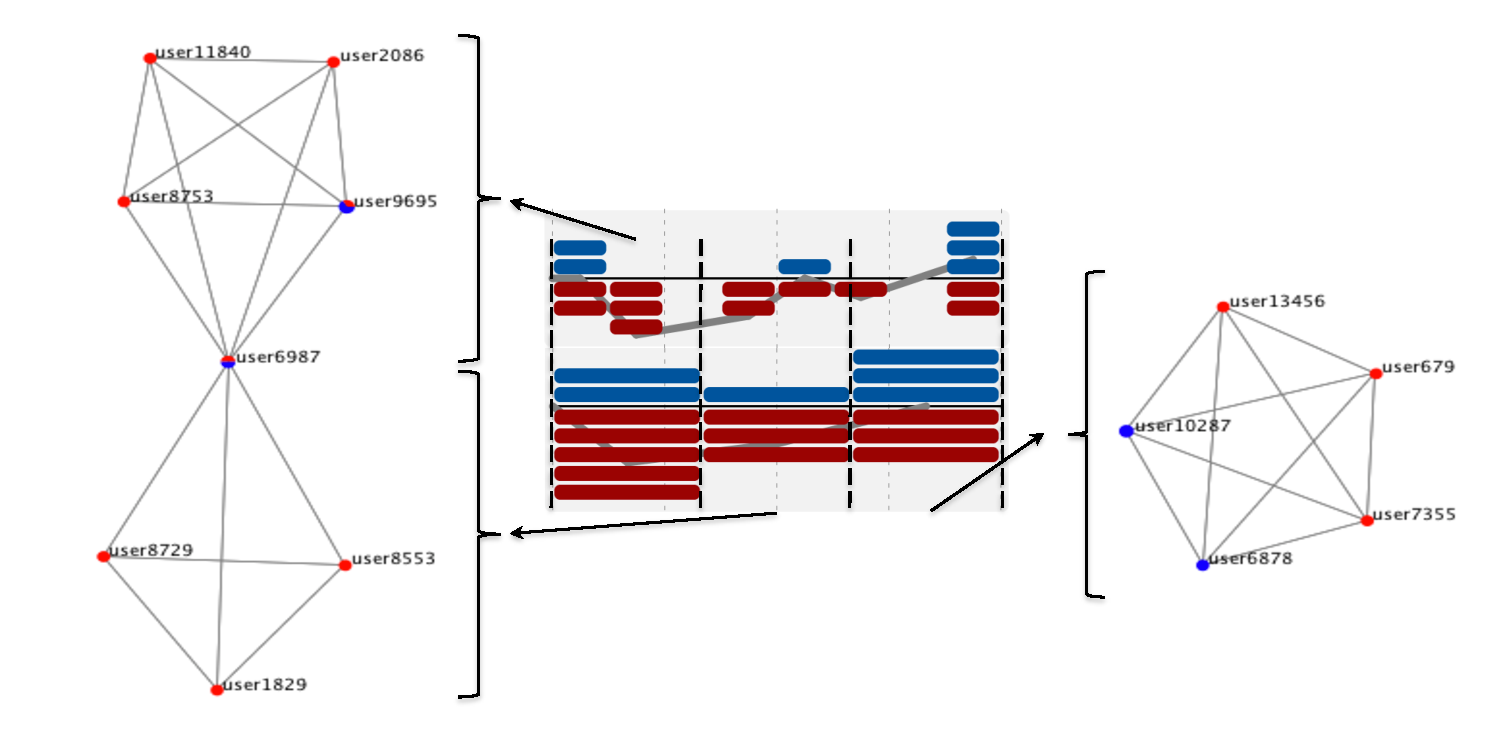
\includegraphics[width=0.8\columnwidth]{img/example-sn2}
\caption{Example of a requirement discussion's social network}
\label{fig:example-sn}
\end{figure}

In this example, the user might conclude that there is no single person who is coordinating the analysis and work related to this requirement, because there is no one actor who participates in all relevant time intervals.
The user decides to assign this responsibility to an experienced developer.

\subsection{Who is knowledgeable about a given topic?}

Integrating the right persons into the loop for an important feature is a crucial ability for managers.
To support managers in this task, \viss\ distinguishes between two types of knowledge: (i) domain knowledge that shows in discussion events related to clarification and (ii) implementation specific knowledge that shows in other discussion events.
\begin{enumerate}
\item The user selects a number of requirements that relate to a feature or higher-level topic. 
\item \viss\ creates the social networks generated from requirement discussions and displays them in a single large network (see Figure \ref{fig:example-sn-large}).
\item Based on the pie charts in the social network, the manager identifies candidates with a balanced percentage of clarification and implementation communication.
\item The user looks for central developers. 
\end{enumerate}
\begin{figure}
\centering
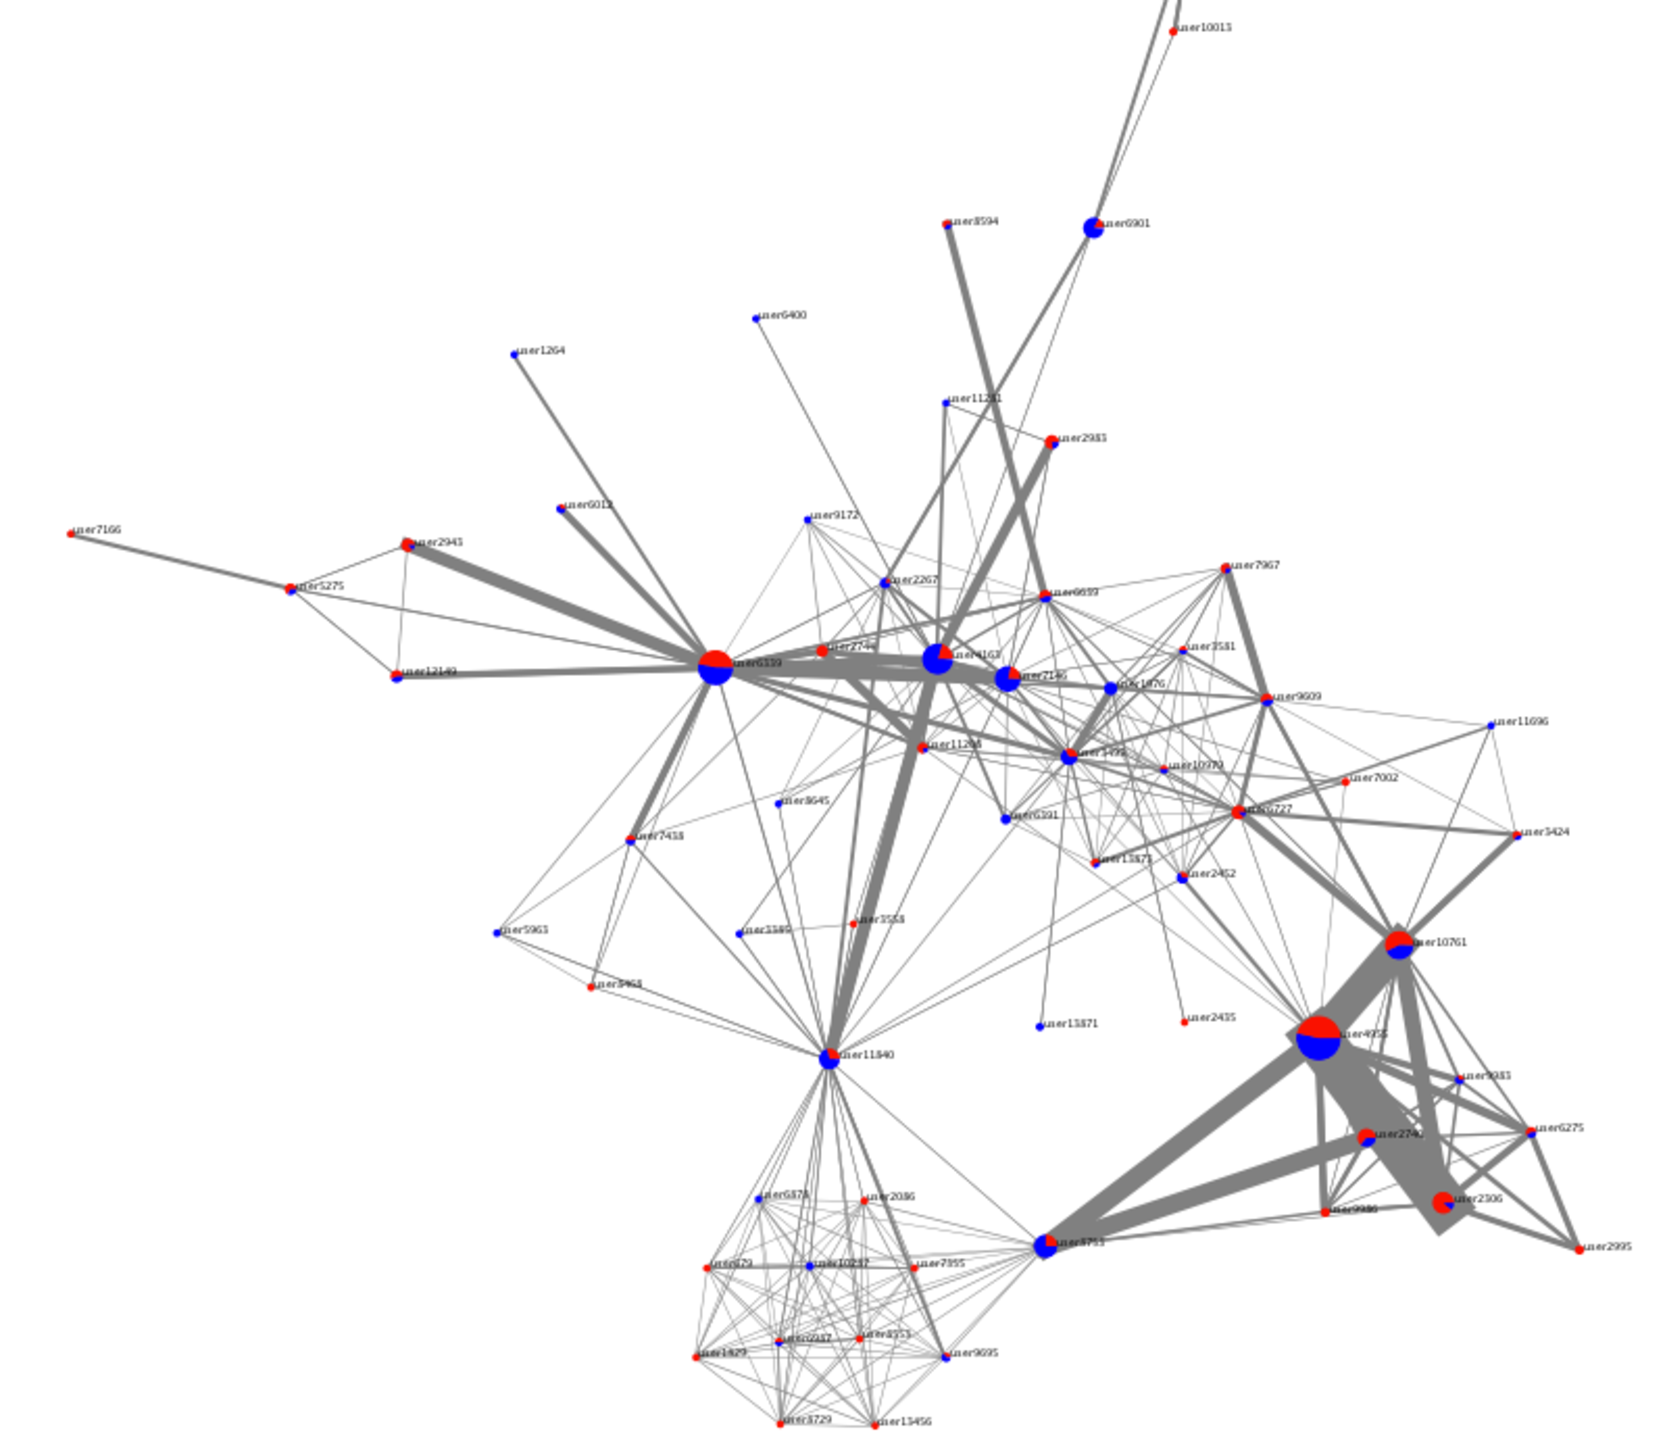
\includegraphics[width=0.8\columnwidth]{img/example-sn-large}
\caption{Example of a social network for a set of requirement discussions. %
%Pie charts (nodes) show the percentage of clarification (red) of developers.
}
\label{fig:example-sn-large}
\end{figure}
Central actors with many connections might already have a very high workload, but there exist good candidates that are less central and connect two subnets.
